% !TeX root = ../../../main.tex

The strategy adopted in this work in order to
determine the intrinsic charm content of the proton is 
based on the following
observation.
%
The assumption that there is no intrinsic charm
amounts to the assumption
that all 4FNS PDFs are determined~\cite{Collins:1986mp} using
perturbative matching conditions~\cite{pdfnnlo} in terms of 
3FNS PDFs
that do not include
a charm \pdf.
%
However, these perturbative matching conditions are
actually given by a square matrix that also includes a 3FNS charm
\pdf.
%
So the assumption of no intrinsic charm amounts to the assumption
that if the 4FNS PDFs are transformed back to the 3FNS, the 3FNS charm
\pdf is found to vanish. Hence, intrinsic charm is by definition the
deviation from zero of the 3FNS charm \pdf~\cite{Ball:2015dpa}. Note
that whereas the 3FNS charm \pdf is purely intrinsic, while the 4FNS
charm \pdf includes both an intrinsic and a perturbative
 radiative component, the
4FNS intrinsic component is not equal to the 3FNS charm \pdf, since
matching conditions reshuffle all PDFs among each other. 

Intrinsic charm can then be determined through the following two steps,
summarized in Fig.~\ref{fig:ic/strategy}. 
First, all the PDFs, including the charm \pdf, are parametrized 
in the 4FNS at an input scale $Q_0$ and evolved 
using \nnlo perturbative QCD to   $Q \not = Q_0$.
%
These evolved PDFs can be used to 
compute physical cross-sections, also at \nnlo, which then are
compared to a global dataset of experimental measurements.
%
The result of this first step in our procedure is 
a Monte Carlo (MC) representation
of the probability distribution for the 4FNS PDFs at the input
parametrization scale $Q_0$.

Next, this 4FNS charm \pdf is transformed to the 3FNS at some scale matching scale
$Q_c$.
%
Note that the choice of both $Q_0$ and $Q_c$ are immaterial. The former
because perturbative evolution is invertible, so
results for the PDFs do not depend on the choice of
parametrization scale $Q_0$. The latter because 
the 3FNS charm is scale independent, so it does not depend on the
value of $Q_c$.
Both statements of course hold up to fixed perturbative accuracy, and
are violated by MHO corrections.
%
In practice, we parametrize PDFs at the scale
$Q_0=$~1.65~GeV and perform the inversion at a scale
chosen equal to the charm mass $Q_c=m_c=1.51$~GeV.

The scale-independent 3FNS charm \pdf is then the sought-for intrinsic
charm.

%%%%%%%%%%%%%%%%%%%%%%%%%%%%%%%%%%%%%%%%%%%%
\begin{figure}[h]
\begin{center}
  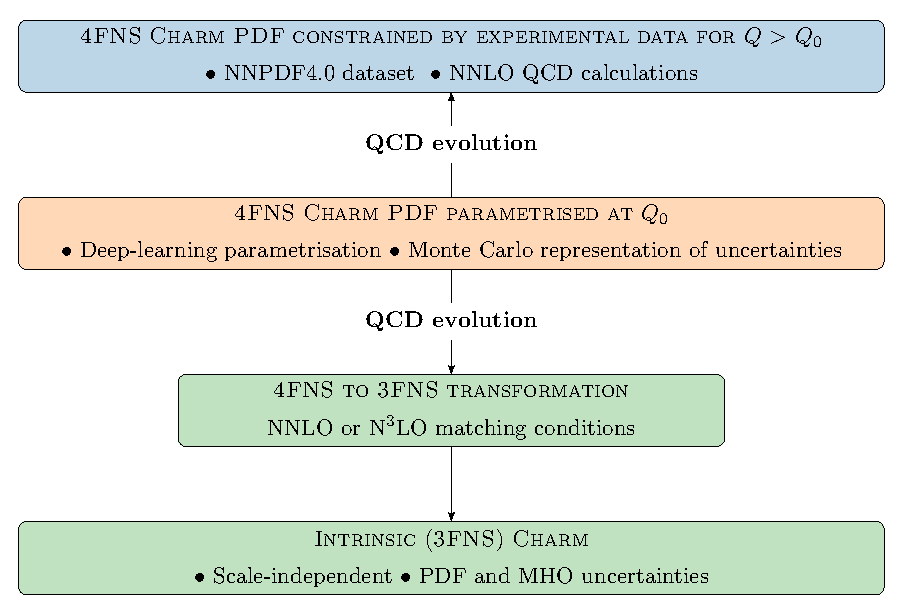
\includegraphics[width=0.8\textwidth]{ch-ic/strategy.pdf}
 \end{center}
\vspace{-0.2cm}
\caption{The 4FNS charm \pdf is parametrized  at $Q_0$
  and evolved to all  $Q$, where it is  constrained by the NNPDF4.0
  global dataset. 
  %
 Subsequently, it is transformed to the 3FNS where (if nonzero) it
 provides the intrinsic charm component.
  \label{fig:ic/strategy}
}
\end{figure}
%%%%%%%%%%%%%%%%%%%%%%%%%%%%%%%%%%%%%%%%%%%%

\paragraph{Global QCD analysis.}
%
The 4FNS charm \pdf and its associated
uncertainties is determined by means of a global QCD analysis
within the NNPDF4.0 framework.
%
All PDFs, including the charm \pdf, are  parametrized at $Q_0=1.65$ GeV in 
a model-independent manner using a neural network, which is fitted to data using 
supervised machine learning techniques.
The Monte Carlo replica method
is deployed to ensure a faithful uncertainty estimate.
%
Specifically, we express the 4FNS total charm \pdf ($c^+=c+\bar{c}$)  in terms of the output neurons associated to the quark singlet $\Sigma$ and non-singlet $T_{15}$
distributions, see Sect.~3.1 of~\cite{Ball:2021leu}, as
\begin{equation}
\label{eq:ic/fitted_charm_param}
xc^+(x,Q_0;{\boldsymbol \theta}) =
\left( x^{\alpha_{\Sigma}}(1-x)^{\beta_{\Sigma}} \textrm{ NN}_{\Sigma}(x,{\boldsymbol \theta})-
x^{\alpha_{T_{15}}}(1-x)^{\beta_{T_{15}}} \textrm{ NN}_{T_{15}}(x,{\boldsymbol \theta})
\right)/4 \, ,
\end{equation}
where $\textrm{NN}_{i}(x,{\boldsymbol \theta})$ is the $i$-th output neuron of
a neural network with input $x$ and  parameters ${\boldsymbol \theta}$, and 
$\left(\alpha_i,\beta_i\right)$ are preprocessing exponents.
%
A crucial feature of Eq.~(\ref{eq:ic/fitted_charm_param}) is that no \textit{
ad hoc} specific model assumptions are used: the shape and size of
$xc^+(x,Q_0)$ are entirely determined from experimental data.
%
Hence, our determination of the 4FNS fitted charm \pdf, and thus of the intrinsic charm, is unbiased.
%

%%%%%%%%%%%%%%%%%%%%%%%%%%%%%%%%%%%%%%%%%%%%
\begin{figure}[t]
\begin{center}
  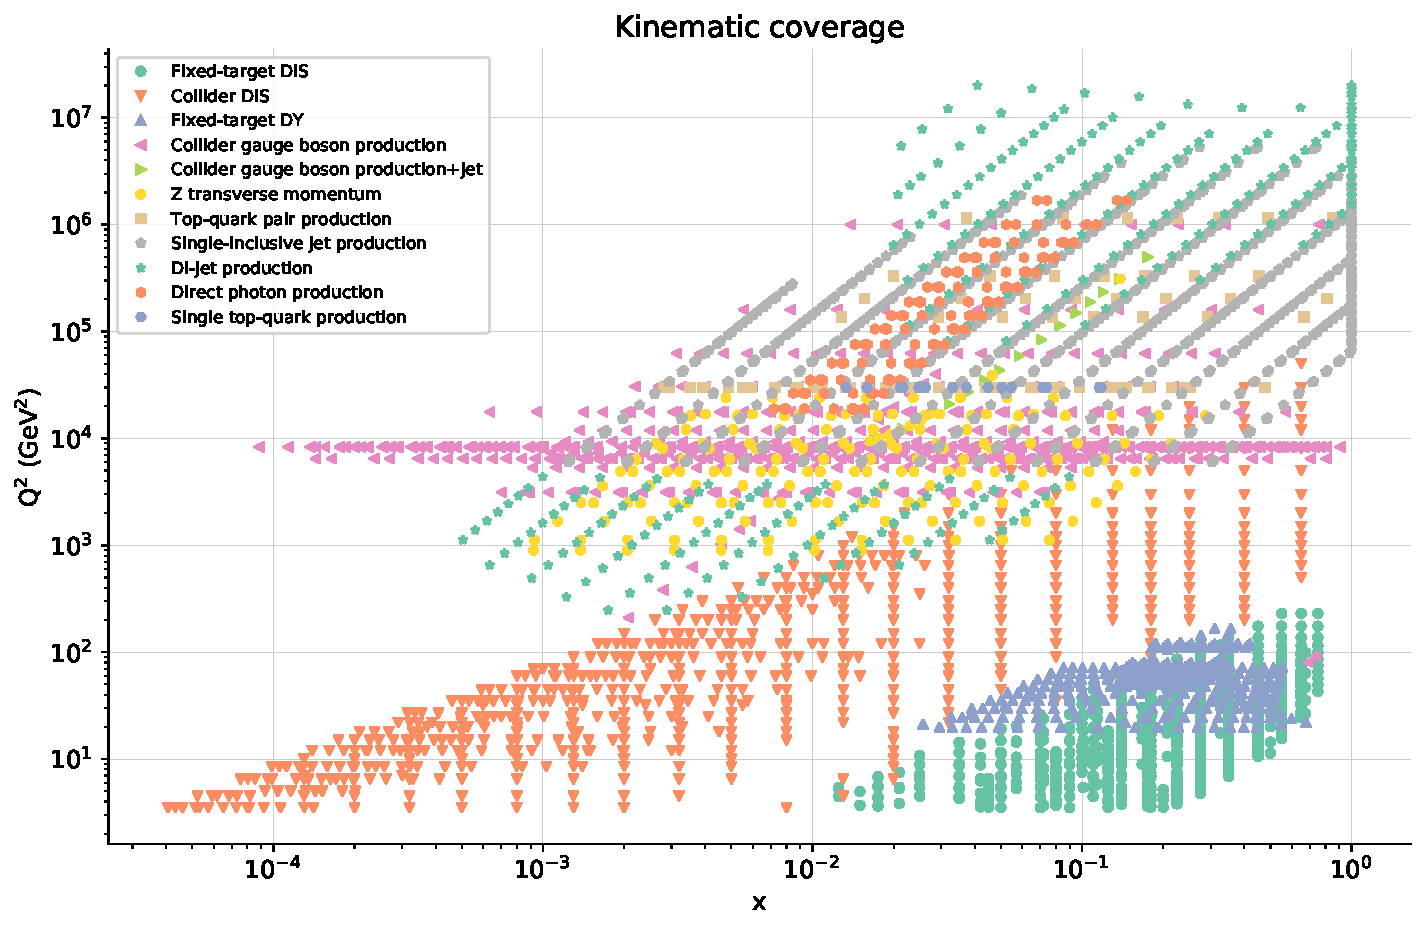
\includegraphics[width=1.0\textwidth]{ch-ic/kinplot.pdf}
 \end{center}
\vspace{-0.8cm}
\caption{The kinematic coverage in the $(x,Q)$ plane
  covered by the 4618 cross-sections used for the
  determination of the charm \pdf in the present work.
  %
  These cross-sections have been classified into the main different
  types of processes entering the global analysis.
  \label{fig:ic/kinplot}
}
\end{figure}
%%%%%%%%%%%%%%%%%%%%%%%%%%%%%%%%%%%%%%%%%%%%

The neural network parameters ${\boldsymbol \theta}$ in
Eq.~(\ref{eq:ic/fitted_charm_param})
are determined by fitting an extensive global dataset that consists of 4618 
cross-sections from a wide range of different processes, measured over
the years in a variety of fixed-target and collider experiments  (see~\cite{Ball:2021leu} for a complete list).
%
Fig.~\ref{fig:ic/kinplot} displays the kinematic coverage in the $(x,Q)$ plane
covered by these cross-sections, where $Q$ is
the  scale, and  $x$ is
the parton momentum fraction that correspond to leading-order kinematics.
%
Many of these processes provide direct or indirect sensitivity 
to the charm content of the proton.
%
Particularly important constraints come from $W$ and $Z$ production from 
\atlas, \cms, and \lhcb as well as from
neutral and charged current deep-inelastic 
scattering (DIS) structure functions from HERA.
%
The 4FNS  PDFs at the input scale $Q_0$ are related
to experimental measurements at $Q \not =Q_0$ by means of \nnlo QCD calculations, including
the FONLL-C general-mass scheme for DIS~\cite{Forte:2010ta} generalized to 
allow for fitted charm~\cite{Ball:2015tna}.

We have verified (see SI
\cref{app:ic/charm_stability_4fns,app:ic/charm_stability_3fns}) that the
determination of 4FNS charm \pdf \cref{eq:ic/fitted_charm_param} and the ensuing
3FNS intrinsic charm \pdf are  stable upon variations of methodology (\pdf
parametrization basis), input dataset, and values of Standard Model parameters
(the charm mass).
We have also studied the stability of our results upon replacing the
current NNPDF4.0 methodology~\cite{Ball:2021leu} with the previous
NNPDF3.1 methodology~\cite{NNPDF:2017mvq}. It turns out that results
are  perfectly consistent. Indeed, the old methodology leads to somewhat larger
uncertainties, corresponding to a moderate reduction of the local statistical
significance for intrinsic charm, and to a central value which is
within the smaller  error band of our current result.


A determination in which the vanishing of intrinsic charm is
imposed has also been performed.
%
In this case, the fit quality significantly
deteriorates: the values of the $\chi^2$ per data point of 1.162,
1.26, and 1.22 for total, Drell-Yan, 
and neutral-current DIS data respectively, found when fitting charm, are 
increased to 1.198, 1.31, 1.28 when the vanishing of intrinsic charm
is imposed.
%
The absolute worsening of the total $\chi^2$ when the vanishing of intrinsic charm is imposed is therefore
of 166 units, corresponding to
a $2\sigma$ effects in units of $\sigma_{\chi^2}= \sqrt{2n_\textrm{ dat}}$.

\paragraph{Calculation of the 3FNS charm \pdf.}
%
The Monte Carlo representation of the probability distribution associated to
the 4FNS charm \pdf determined by the global
analysis contains an intrinsic component mixed with a perturbatively
generated contribution, with the latter
becoming larger in the $x\lsim 0.1$ region as the scale $Q$ is increased.
%
In order to extract the intrinsic component, 
we transform PDFs to the 3FNS at the scale $Q_c=m_c=1.51$~GeV using
\textsc{\small EKO}, a novel \textsc{\small Python} open source
\pdf evolution framework (see  SI Sect.~\ref{app:ic/eko}).
%
In its current implementation, \textsc{\small EKO} performs  QCD 
evolution of PDFs to any scale
up to \nnlo. For
the sake of the current analysis, \nnnlo matching conditions have also
been implemented, by 
using  the results
of~\cite{Bierenbaum:2009zt,Bierenbaum:2009mv,Ablinger:2010ty,Ablinger:2014vwa,Ablinger:2014uka,Behring:2014eya,Ablinger_2014,Ablinger:2014nga,Blumlein:2017wxd}
for $\mathcal{O}(\alpha_s^3)$ operator matrix elements~
so that the direct and inverse transformations from the 3FNS to the
4FNS can be performed at one order
higher.
%
The \nnnlo contributions to the matching conditions are a subset of
the full \nnnlo terms that would be required to perform a \pdf determination
 to one higher perturbative order, and would
also include currently unknown
\nnnlo contributions to QCD evolution. Therefore, our results have 
\nnlo accuracy and we can only use the  \nnnlo contributions to the
 $\mathcal{O}(\alpha_s^3)$ corrections to the
heavy quark matching
matching conditions as a way to estimate the 
the size of the missing higher orders. 
Indeed, these corrections have a very 
significant impact on the
perturbatively generated component, see SI Sect.~\ref{app:ic/consistency}.
%
They become large for $x \lsim 0.1$, which coincides with the region
dominated by the perturbative component of the charm \pdf,
  and are relatively small for the valence region
  where intrinsic charm dominates.
  
\paragraph{$Z$ production in association with charm-tagged jets.}
%
The production of $Z$ bosons in association with charm-tagged jets (or alternatively,
with identified $D$ mesons) at the \lhc is directly sensitive to the charm content
of the proton via the dominant $gc \to Zc$ partonic scattering process.
%
Measurements of this process at  the forward rapidities covered by the
\lhcb acceptance provide access to the large-$x$ region where the intrinsic 
contribution is expected to dominate.
%
This is in contrast with the corresponding measurements from \atlas and \cms,
which only become sensitive to intrinsic charm
at rather larger values of $p_T^Z$ than those
currently accessible experimentally.

We have obtained  theoretical predictions for $Z$+charm production
at \lhcb with NNPDF4.0, based on
\nlo QCD calculations using
\textsc{\small POWHEG-BOX} 
interfaced to \textsc{\small Pythia8}
with the Monash 2013 tune for showering,
hadronization, and underlying event.
%
Acceptance requirements and event selection follow the \lhcb analysis,
where in particular charm jets are defined as those anti-$k_T$ $R=0.5$ jets
containing a reconstructed charmed hadron.
%
The ratio between $c$-tagged and untagged $Z$+jet events can then
be compared with the \lhcb measurements
\begin{equation}
  \mathcal{R}_j^c(y_Z) \equiv \frac{N(c~\textrm{ tagged~jets};y_Z)}{ 
    N(\textrm{ jets};y_Z)} =
  \frac{\sigma(pp\to Z+\textrm{ charm~ jet};y_Z)}{\sigma(pp \to Z+\textrm{ jet};y_Z)} \, ,
\end{equation}
as a function of the $Z$ boson rapidity $y_Z$ (see SI Sect.~\ref{sec:ic/zcharm} for details).
%
The more forward the rapidity $y_{Z}$, the higher the values of the charm
momentum $x$ being probed.
%
Furthermore, we have also included the \lhcb measurements in the global \pdf
determination by means of the Bayesian reweighting (see SI
Sect.~\ref{sec:ic/zcharm}).
